\documentclass[12pt]{article}

\usepackage[english]{babel}
\usepackage[utf8]{inputenc}
\usepackage[top=2cm, left=2cm, right=2cm, bottom=2cm]{geometry}
\usepackage[document]{ragged2e}
\usepackage{tikz,minted,times}

\setlength\parindent{0pt}
\sloppy
\usetikzlibrary{automata,positioning,arrows,fit}
\tikzset{node distance=2.5cm,every state/.style={semithick,fill=gray!10},initial text={},double distance=2pt,every edge/.style={draw,->,>=stealth,auto,semithick}}
\usemintedstyle{colorful}

\title{COMP SCI 7411 Event Driven Computing Practice 3 Plan}
\author{Tinson Lai \\ a1812422}
\date{}

\begin{document}

\maketitle

Due to the constraint that train will not change direction, the following routes are the only options for trains entering the system.

\begin{itemize}
  \item Train entering from $1$ going east

    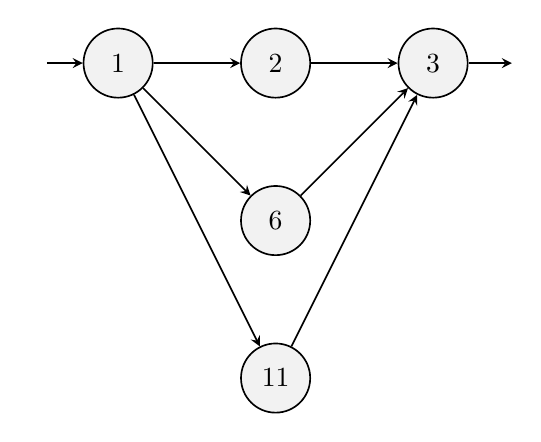
\begin{tikzpicture}
      \node[state, initial] at (0, 4) (1){1};
      \node[state] at (2, 4) (2){2};
      \node[state] at (2, 2) (6){6};
      \node[state] at (2, 0) (11){11};
      \node[state] at (4, 4) (3){3};

      \draw

      (1) edge (2)
      (1) edge (6)
      (1) edge (11)

      (2) edge (3)
      (6) edge (3)
      (11) edge (3)

      (3) edge +(1, 0)

      ;
    \end{tikzpicture}
  \item Train entering from $4$ going east

    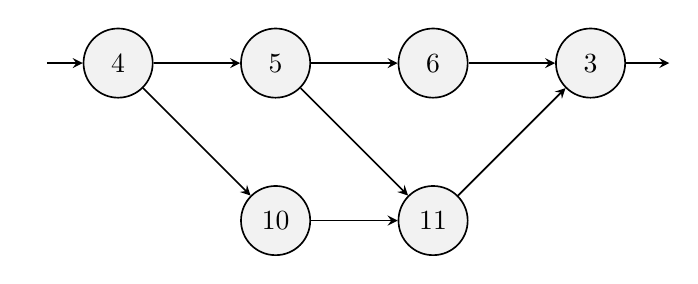
\begin{tikzpicture}
      \node[state, initial] at (0, 2) (4){4};
      \node[state] at (2, 2) (5){5};
      \node[state] at (4, 2) (6){6};
      \node[state] at (6, 2) (3){3};
      \node[state] at (2, 0) (10){10};
      \node[state] at (4, 0) (11){11};

      \draw

      (4) edge (5)
      (4) edge (10)

      (5) edge (6)
      (5) edge (11)
      (10) edge (11)

      (6) edge (3)
      (11) edge (3)

      (3) edge +(1, 0)

      ;
    \end{tikzpicture}
  \item Train entering from $8$ going west

    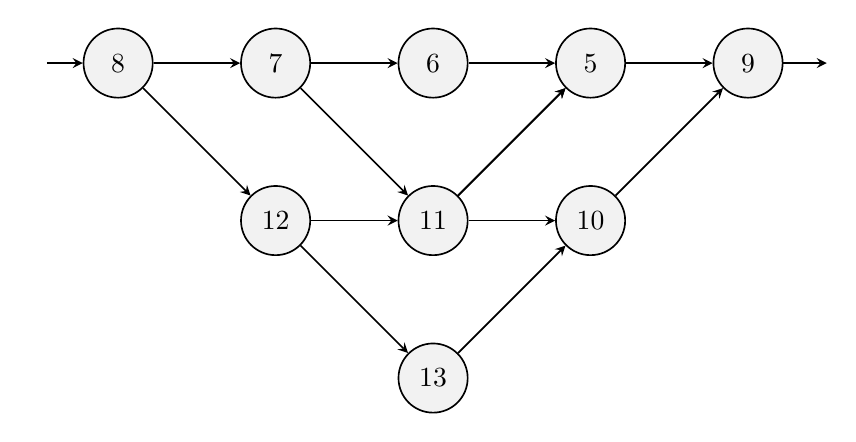
\begin{tikzpicture}
      \node[state, initial] at (0, 4) (8){8};
      \node[state] at (2, 4) (7){7};
      \node[state] at (4, 4) (6){6};
      \node[state] at (6, 4) (5){5};
      \node[state] at (8, 4) (9){9};
      \node[state] at (2, 2) (12){12};
      \node[state] at (4, 2) (11){11};
      \node[state] at (6, 2) (10){10};
      \node[state] at (4, 0) (13){13};

      \draw

      (8) edge (7)
      (8) edge (12)

      (7) edge (6)
      (7) edge (11)

      (12) edge (11)
      (12) edge (13)

      (11) edge (5)
      (11) edge (10)

      (13) edge (10)

      (6) edge (5)
      (11) edge (5)

      (5) edge (9)
      (10) edge (9)

      (9) edge +(1, 0)

      ;
    \end{tikzpicture}
\end{itemize}

In the following sections, I will use the following notations in the Petri Net, where in the Petri Net tuple $N=\left(P,T,A,W,I\right)$

\begin{itemize}
  \item ($P$) $p_i$ refers to track $i$ when it's empty. $p_{i,e}$ or $p_{i,w}$ refers to track $i$ with a east direction ($e$) or west direction ($w$) train on it. This is a necessary notation to avoid deadlock.  All $p_i$ with $p_{i,e}$ and $p_{i,w}$ forms different buffers in the Petri Net.
  \item ($P$) $d_i$ refers to a dispatcher, where only $d_1$, $d_4$ and $d_8$ are available as trains can only enter the system from these tracks. They also act as producers in the Petri Net as well.
  \item ($P$) $o_i$ refers to the outgoing track, where only $o_3$ and $o_9$ are available as trains can only exit the system from these tracks. They also act as consumers in the Petri Net as well.
  \item ($T$) $e_{i,j}$ or $w_{i,j}$ refers to a move from track $i$ to track $j$ in the direction of east ($e$) or west ($w$).
  \item $W$ will always be one for all transitions.
  \item ($I$) All $p_i$, $d_i$ and $o_i$ will be an initial states as implied by the definition of producer, consumer and buffer. It is also obvious that the initial system will be completely empty, so the initial state should be neither $p_{i,e}$ nor $p_{1,w}$ but $p_i$.
\end{itemize}

\section{Entering from $1$}

There will be no chance of deadlock in any routes available for train entering from 1, as the intermediate tracks $2$, $6$ and $11$ can reach track $3$ directly so trains in this part can safely pass through any intersections involved in this part.. The only requirement for the move is that the destination track needs to be empty.

\subsection{$1 \rightarrow 2 \rightarrow 3$}

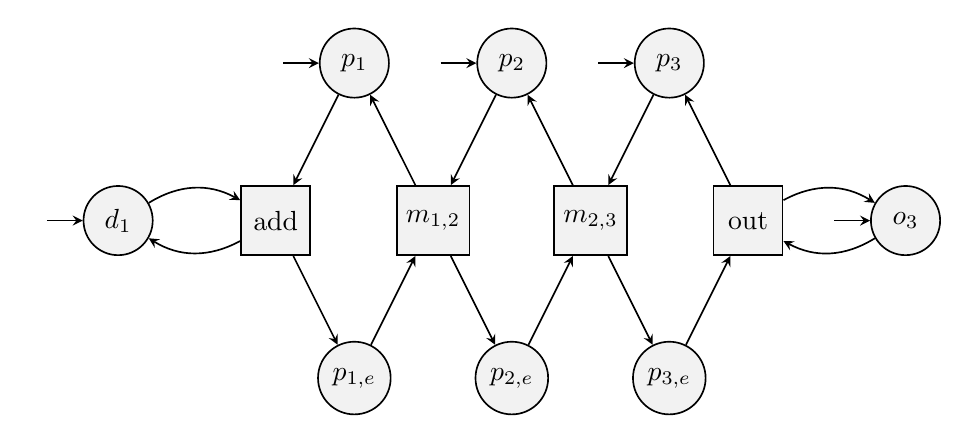
\begin{tikzpicture}
  \node[state, initial] at (0, 2) (d1){$d_1$};
  \node[state, initial] at (10, 2) (o3){$o_3$};

  \node[state, initial] at (3, 4) (p1){$p_1$};
  \node[state, initial] at (5, 4) (p2){$p_2$};
  \node[state, initial] at (7, 4) (p3){$p_3$};

  \node[state] at (3, 0) (p1_e){$p_{1,e}$};
  \node[state] at (5, 0) (p2_e){$p_{2,e}$};
  \node[state] at (7, 0) (p3_e){$p_{3,e}$};

  \node[state, rectangle] at (2, 2) (add){add};
  \node[state, rectangle] at (4, 2) (m1_2){$m_{1,2}$};
  \node[state, rectangle] at (6, 2) (m2_3){$m_{2,3}$};
  \node[state, rectangle] at (8, 2) (out){out};

  \draw

  (d1) edge[bend left] (add)
  (add) edge[bend left] (d1)
  (p1) edge (add)
  (add) edge (p1_e)

  (p1_e) edge (m1_2)
  (m1_2) edge (p1)
  (p2) edge (m1_2)
  (m1_2) edge (p2_e)

  (p2_e) edge (m2_3)
  (m2_3) edge (p2)
  (p3) edge (m2_3)
  (m2_3) edge (p3_e)


  (p3_e) edge (out)
  (out) edge (p3)
  (o3) edge[bend left] (out)
  (out) edge[bend left] (o3)

  ;
\end{tikzpicture}

\subsection{$1 \rightarrow 6 \rightarrow 3$}

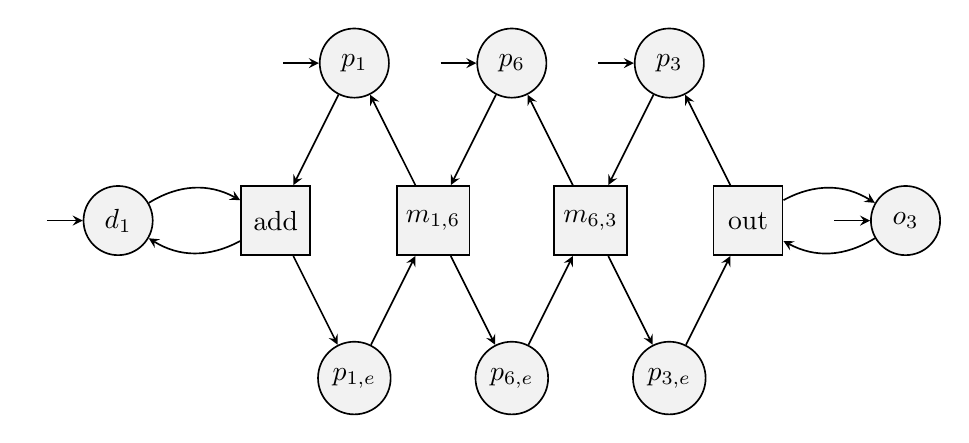
\begin{tikzpicture}
  \node[state, initial] at (0, 2) (d1){$d_1$};
  \node[state, initial] at (10, 2) (o3){$o_3$};

  \node[state, initial] at (3, 4) (p1){$p_1$};
  \node[state, initial] at (5, 4) (p6){$p_6$};
  \node[state, initial] at (7, 4) (p3){$p_3$};

  \node[state] at (3, 0) (p1_e){$p_{1,e}$};
  \node[state] at (5, 0) (p6_e){$p_{6,e}$};
  \node[state] at (7, 0) (p3_e){$p_{3,e}$};

  \node[state, rectangle] at (2, 2) (add){add};
  \node[state, rectangle] at (4, 2) (m1_6){$m_{1,6}$};
  \node[state, rectangle] at (6, 2) (m6_3){$m_{6,3}$};
  \node[state, rectangle] at (8, 2) (out){out};

  \draw

  (d1) edge[bend left] (add)
  (add) edge[bend left] (d1)
  (p1) edge (add)
  (add) edge (p1_e)

  (p1_e) edge (m1_6)
  (m1_6) edge (p1)
  (p6) edge (m1_6)
  (m1_6) edge (p6_e)

  (p6_e) edge (m6_3)
  (m6_3) edge (p6)
  (p3) edge (m6_3)
  (m6_3) edge (p3_e)


  (p3_e) edge (out)
  (out) edge (p3)
  (o3) edge[bend left] (out)
  (out) edge[bend left] (o3)

  ;
\end{tikzpicture}

\subsection{$1 \rightarrow 11 \rightarrow 3$}

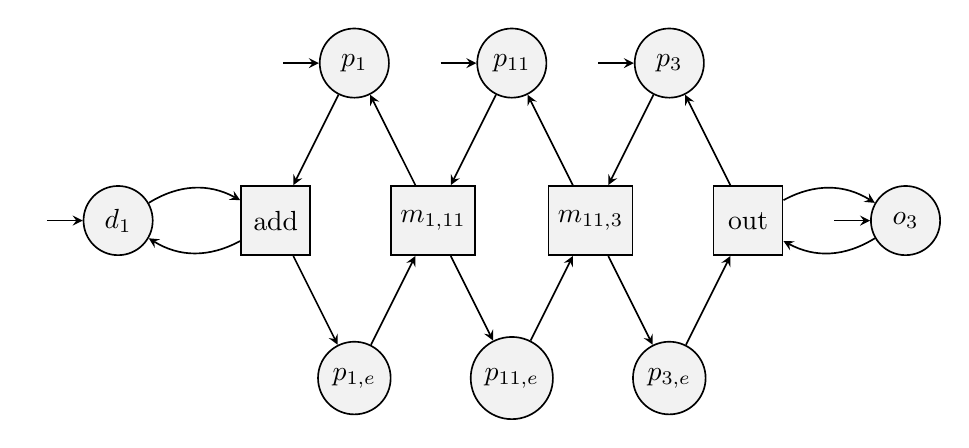
\begin{tikzpicture}
  \node[state, initial] at (0, 2) (d1){$d_1$};
  \node[state, initial] at (10, 2) (o3){$o_3$};

  \node[state, initial] at (3, 4) (p1){$p_1$};
  \node[state, initial] at (5, 4) (p11){$p_{11}$};
  \node[state, initial] at (7, 4) (p3){$p_3$};

  \node[state] at (3, 0) (p1_e){$p_{1,e}$};
  \node[state] at (5, 0) (p11_e){$p_{11,e}$};
  \node[state] at (7, 0) (p3_e){$p_{3,e}$};

  \node[state, rectangle] at (2, 2) (add){add};
  \node[state, rectangle] at (4, 2) (m1_11){$m_{1,11}$};
  \node[state, rectangle] at (6, 2) (m11_3){$m_{11,3}$};
  \node[state, rectangle] at (8, 2) (out){out};

  \draw

  (d1) edge[bend left] (add)
  (add) edge[bend left] (d1)
  (p1) edge (add)
  (add) edge (p1_e)

  (p1_e) edge (m1_11)
  (m1_11) edge (p1)
  (p11) edge (m1_11)
  (m1_11) edge (p11_e)

  (p11_e) edge (m11_3)
  (m11_3) edge (p11)
  (p3) edge (m11_3)
  (m11_3) edge (p3_e)


  (p3_e) edge (out)
  (out) edge (p3)
  (o3) edge[bend left] (out)
  (out) edge[bend left] (o3)

  ;
\end{tikzpicture}

\section{Entering from $4$}

Unlike trains coming from $1$, it is possible for trains coming from $4$ and $8$ to entre a deadlock situation when $5$ and $10$ both have a train driving east but both $6$ and $11$ have a train driving west. It is important to ensure that one of the tracks is empty, or at least, one of the tracks having a train travelling in a correct direction which can escape from the congestion.

\section{Entering from $8$}

\section{Priority}

Despite the design above, it's important to introduce the concept of priority to prioritise the selection of track in each intersection. This can avoid blocking one of the train entrance permanently when the system is busy. This is especially important to the outgoing track from $3$ as trains entering from $1$ and $4$ will merge into track $3$.

\end{document}
